\chapter{Simulation} \label{cha:sim}

\clearpage

\section{WrightSim}  % ===================================================================

This section was originally published in Scipy Proceedings 2018 \cite{SundenKyleFoster2018a}

\hypertarget{wrightsim-using-pycuda-to-simulate-multidimensional-spectra}{%
\subsection{\texorpdfstring{\texttt{WrightSim}: Using PyCUDA to Simulate
Multidimensional
Spectra}{WrightSim: Using PyCUDA to Simulate Multidimensional Spectra}}\label{wrightsim-using-pycuda-to-simulate-multidimensional-spectra}}

Nonlinear multidimensional spectroscopy (MDS) is a powerful experimental
technique used to interrogate complex chemical systems. MDS promises to
reveal energetics, dynamics, and coupling features of and between the
many quantum-mechanical states that these systems contain. In practice,
simulation is typically required to connect measured MDS spectra with
these microscopic physical phenomena. We present an open-source Python
package, \texttt{WrightSim}, designed to simulate MDS. Numerical
integration is used to evolve the system as it interacts with several
electric fields in the course of a multidimensional experiment. This
numerical approach allows \texttt{WrightSim} to fully account for finite
pulse effects that are commonly ignored. \texttt{WrightSim} is made up
of modules that can be exchanged to accommodate many different
experimental setups. Simulations are defined through a Python interface
that is designed to be intuitive for experimentalists and theorists
alike. We report several algorithmic improvements that make
\texttt{WrightSim} faster than previous implementations. We demonstrated
the effect of parallelizing the simulation, both with CPU
multiprocessing and GPU (CUDA) multithreading. Taken together,
algorithmic improvements and parallelization have made
\texttt{WrightSim} multiple orders of magnitude faster than previous
implementations. \texttt{WrightSim} represents a large step towards the
goal of a fast, accurate, and easy to use general purpose simulation
package for multidimensional spectroscopy. To our knowledge,
\texttt{WrightSim} is the first openly licensed software package for
these kinds of simulations. Potential further improvements are
discussed.

Simulation, spectroscopy, PyCUDA, numerical integration, Quantum
Mechanics, multidimensional

\hypertarget{introduction}{%
\subsubsection{Introduction}\label{introduction}}

Nonlinear multidimensional spectroscopy (MDS) is an increasingly
important analytical technique for the analysis of complex chemical
material systems. MDS can directly observe fundamental physics that are
not possible to record in any other way. With recent advancements in
lasers and optics, MDS experiments are becoming routine. Applications of
MDS in semiconductor photophysics \cite{CzechKyleJonathan2015a}, medicine
\cite{Fournier_2009}, and other domains \cite{Petti_2018} are
currently being developed. Ultimately, MDS may become a key research
tool akin to multidimensional nuclear magnetic resonance spectroscopy.
\cite{PakoulevAndreiV2009a}

A generic MDS experiment involves exciting a sample with multiple pulses
of light and measuring the magnitude of the sample response (the
signal). The dependence of this signal on the properties of the
excitation pulses (frequency, delay, fluence, polarization etc.)
contains information about the microscopic physics of the material.
However, this information cannot be directly "read off" of the spectrum.
Instead, MDS practitioners typically compare the measured spectrum with
model spectra. A quantitative microscopic model is developed based on
this comparison between experiment and theory. Here, we focus on this
crucial modeling step. We present a general-purpose simulation package
for MDS: \texttt{WrightSim}\footnote{Source code available at
  \url{https://github.com/wright-group/WrightSim}, released under MIT
  License.}.

\begin{figure}
\centering
	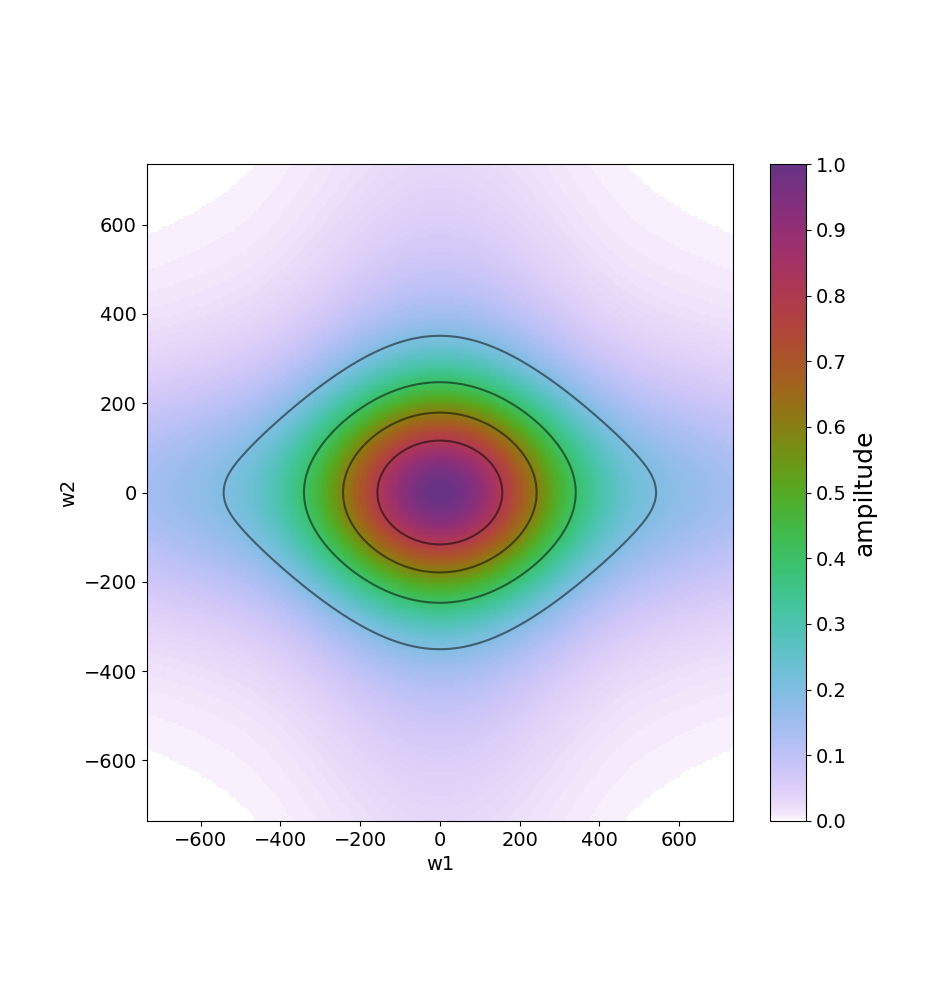
\includegraphics[width=6in]{simulation/images/example_spectrum.png}
\caption{Simulated spectrum at normalized coordinates
\label{sim:fig:examplespectrum}}
\end{figure}

Figure \ref{sim:fig:examplespectrum} is a visualization of a spectrum in
2-dimensional frequency-frequency space. The axes are two different
frequencies for two separate input electric fields. The system that we
have chosen for this simulation is very simple, with a single resonance.
The axes are translated such that there is a resonance around \(0.0\) in
both frequencies. This two-dimensional simulation is representative of
\texttt{WrightSim}'s ability to traverse through many aspects of
experimental space. Every conceivable pulse parameter (delay, fluence,
frequency, chirp etc.) can become an axis in the simulation.

\texttt{WrightSim} is designed with the experimentalist in mind,
allowing users to parameterize their simulations in much the same way
that they would collect a similar spectrum in the laboratory.
\texttt{WrightSim} is modular and flexible. It is capable of simulating
different kinds of MDS, and it is easy to extend to new kinds.

\texttt{WrightSim} uses a numerical integration approach that captures
the full interaction between material and electric field without making
common limiting assumptions. This approach makes \texttt{WrightSim}
flexible, accurate, and interpretable. While the numerical approach we
use is more accurate, it does demand significantly more computational
time. We have focused on performance as a critical component of
\texttt{WrightSim}. Here we report algorithmic improvements which have
significantly decreased computational time (i.e. wall clock time)
relative to prior implementations. We also discuss parallelization
approaches we have taken, and show how the symmetry of the simulation
can be exploited. While nascent, \texttt{WrightSim} has already shown
itself to be a powerful tool, greatly improving execution time over
prior implementation.

\hypertarget{a-brief-introduction-of-relevant-quantum-mechanics}{%
\subsubsection{A Brief Introduction of Relevant Quantum
Mechanics}\label{a-brief-introduction-of-relevant-quantum-mechanics}}

This introduction is intended to very quickly introduce \emph{what} is
being done, but not \emph{why}. If you are interested in a more complete
description, please refer to Kohler, Thompson, and Wright.
\cite{KohlerDanielDavid2017a}

\texttt{WrightSim} uses the density matrix formulation of quantum
mechanics. This formulation allows us to describe mixed states
(coherences) which are key players in light-matter-interaction and
spectroscopy. This involves numerically integrating the Liouville-von
Neumann equation \cite{Gibbs1902}. This strategy has been described
before \cite{Gelin_2009}, so we are brief in our description here.

\texttt{WrightSim} calculates multidimensional spectra for a given
well-defined Hamiltonian. We do not make common limiting assumptions
that allow reduction to analytical expressions. Instead, we propagate
all of the relevant density matrix elements, including populations and
coherences, in a numerical integration. This package does \textbf{not}
perform \emph{ab initio} computations. This places \texttt{WrightSim} at
an intermediate level of theory where the Hamiltonian is known, but
accurately computing the corresponding multidimensional spectrum
requires complicated numerical analysis.

Now, we focus on one representative experiment and Hamiltonian. In this
case, we are simulating the interactions of three electric fields to
induce an output electric field. For three fields, there are \(3! = 6\)
possible time orderings for the pulses to interact and create
superpositions or populations in the material system (Figure
\ref{sim:fig:WMELs}, columns). Within each time ordering, there are
several different pathways (Figure \ref{sim:fig:WMELs}, rows). In total,
there are 16 pathways, represented in Figure \ref{sim:fig:WMELs} as a
series of wave mixing energy level (WMEL) diagrams \cite{Lee_1985}.
We are restricting this simulation to have two positive interactions
(solid up arrows or dashed down arrows) and one negative interaction
(dashed up arrow or solid down arrow). Experimentalists isolate this
condition spatially using an aperture. They can isolate the time
orderings by introducing delays between pulses. Simulation allows us to
fully separate each pathway, leading to insight into the nature of
pathway interference in the total signal line shape.

\begin{figure}
\centering
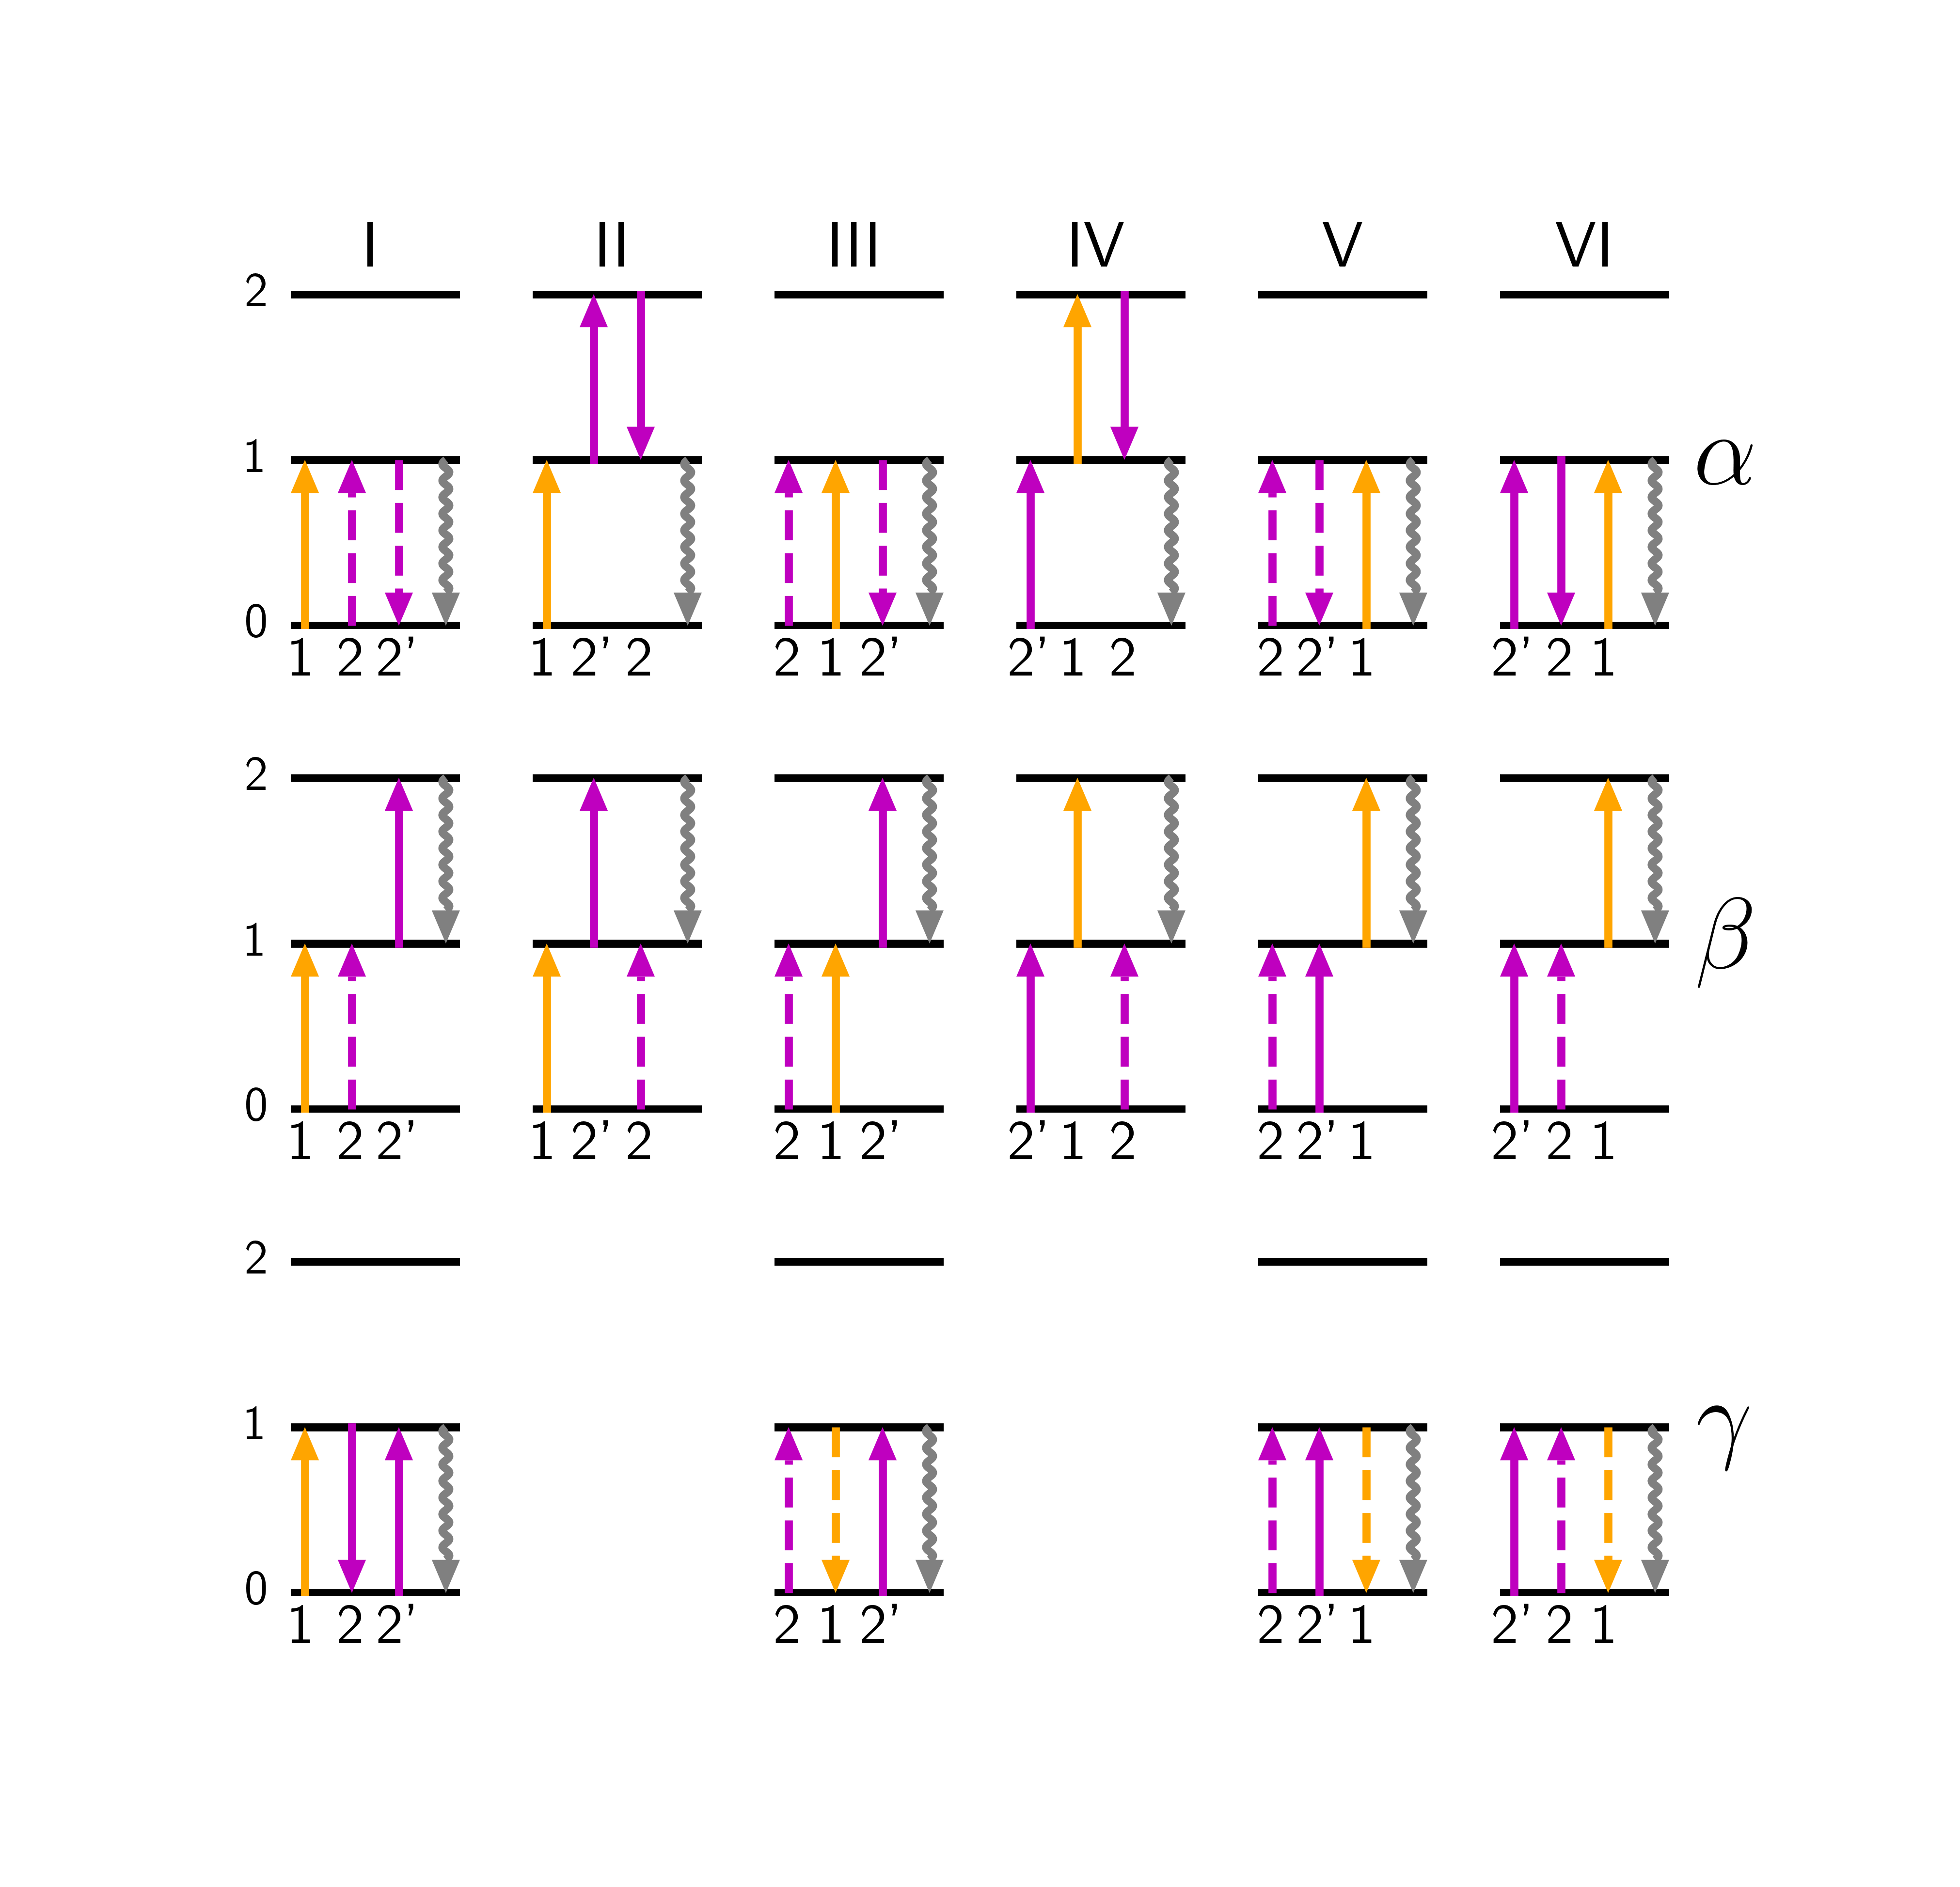
\includegraphics{simulation/images/WMELs.png}
\caption{Independent Liouville pathways simulated. Excitations from
\(\omega_1\) are in yellow, excitations from
\(\omega_2 = \omega_{2^\prime}\) are shown in purple. Figure was
originally published as Figure 1 of Kohler, Thompson, and Wright
\cite{KohlerDanielDavid2017a} \label{sim:fig:WMELs}}
\end{figure}

\begin{figure}
\centering
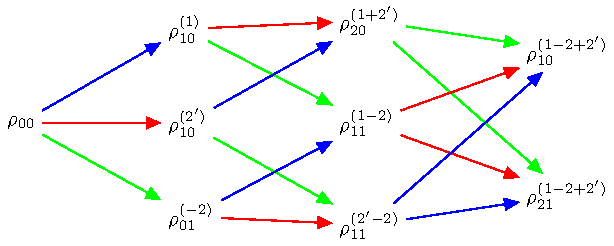
\includegraphics{simulation/images/flow_diagram.pdf}
\caption{Finite state automaton of the interactions with the density
matrix elements. Matrix elements are denoted by their
coherence/population state (the subscript) and the pulses which they
have already interacted with (the superscript). Arrows indicate
interactions with \(\omega_1\) (blue), \(\omega_{2^\prime}\) (red), and
\(\omega_2\) (green). Figure was originally published as Figure S1 of
Kohler, Thompson, and Wright \cite{KohlerDanielDavid2017a} \ref{sim:fig:fsa}}
\end{figure}

Figure \ref{sim:fig:fsa} shows a finite state automaton for the same
system as Figure \ref{sim:fig:WMELs}. The nodes are the density matrix
elements themselves. All pathways start at the ground state
(\(\rho_{00}\)). Encoded within each node is both the quantum mechanical
state and the fields with which the system has already interacted.
Interactions occur along the arrows, which generate density in the
resulting state. Here, the fields must each interact exactly once.
Output is generated by the rightmost two nodes, which have interacted
with all three fields. These nine states represent all possible states
which match the criterion described by the process we are simulating.

We take these nine states and collect them into a state density vector,
\(\overline{\rho}\) (Equation 1.1):

\[\begin{aligned}
\overline{\rho} \equiv
\begin{bmatrix}
\tilde{\rho}_{00} \\
\tilde{\rho}_{01}^{(-2)} \\
\tilde{\rho}_{10}^{(2^\prime)} \\
\tilde{\rho}_{10}^{(1)} \\
\tilde{\rho}_{20}^{(1+2^\prime)} \\
\tilde{\rho}_{11}^{(1-2)} \\
\tilde{\rho}_{11}^{(2^\prime-2)} \\
\tilde{\rho}_{10}^{(1-2+2^\prime)} \\
\tilde{\rho}_{21}^{(1-2+2^\prime)}
\end{bmatrix}
\end{aligned}\]

Next we need to describe the transitions within these states. This is
the Hamiltonian matrix. Since we have nine states in our density vector,
the Hamiltonian is a nine by nine matrix. To simplify representation,
six time dependent variables are defined:

\[\begin{aligned}
\begin{aligned}
A_1 &\equiv& \frac{i}{2}\mu_{10}e^{-i\omega_1\tau_1}c_1(t-\tau_1)e^{i(\omega_1-\omega_{10})t} \\
A_2 &\equiv& \frac{i}{2}\mu_{10}e^{i\omega_2\tau_2}c_2(t-\tau_2)e^{-i(\omega_2-\omega_{10})t} \\
A_{2^\prime} &\equiv& \frac{i}{2}\mu_{10}e^{-i\omega_{2^\prime}\tau_{2^\prime}}c_{2^\prime}(t-\tau_{2^\prime})e^{i(\omega_{2^\prime}-\omega_{10})t} \\
B_1 &\equiv& \frac{i}{2}\mu_{21}e^{-i\omega_1\tau_1}c_1(t-\tau_1)e^{i(\omega_1-\omega_{21})t} \\
B_2 &\equiv& \frac{i}{2}\mu_{21}e^{i\omega_2\tau_2}c_2(t-\tau_2)e^{-i(\omega_2-\omega_{21})t} \\
B_{2^\prime} &\equiv& \frac{i}{2}\mu_{21}e^{-i\omega_{2^\prime}\tau_{2^\prime}}c_{2^\prime}(t-\tau_{2^\prime})e^{i(\omega_{2^\prime}-\omega_{21})t}\end{aligned}
\end{aligned}\]

These variables each consist of a constant factor of \(\frac{i}{2}\), a
dipole moment term (\(\mu_{10|21}\)), an electric field phase and
amplitude (the first exponential term), an envelope function (\(c\), a
Gaussian function here), and a final exponential term which captures the
resonance dependence. These variables can then be used to populate the
matrix:

\[\begin{aligned}
\overline{\overline{Q}} \equiv
\setlength{\arraycolsep}{2pt}
\begin{bmatrix}
    0 & 0 & 0 & 0 & 0 & 0 & 0 & 0 & 0 \\
    -A_2 & -\Gamma_{10} & 0 & 0 & 0 & 0 & 0 & 0 & 0 \\
    A_{2^\prime} & 0 & -\Gamma_{10} & 0 & 0 & 0 & 0 & 0 & 0 \\
    A_1 & 0 & 0 & -\Gamma_{10} & 0 & 0 & 0 & 0 & 0 \\
    0 & 0 & B_1 & B_{2^\prime} & -\Gamma_{20} & 0 & 0 & 0 & 0 \\
    0 & A_1 & 0 & -A_2 & 0 & -\Gamma_{11} & 0 & 0 & 0 \\
    0 & A_{2^\prime} & -A_2 & 0 & 0 & 0 & -\Gamma_{11} & 0 & 0 \\
    0 & 0 & 0 & 0 & B_2 & -2A_{2^\prime} & -2A_1 & -\Gamma_{10} & 0 \\
    0 & 0 & 0 & 0 & -A_2 & B_{2^\prime} & B_1 & 0 & -\Gamma_{21}
\end{bmatrix}
\label{eq:single_Q}
\end{aligned}\]

The \(\Gamma\) values along the diagonal represent loss terms such as
dephasing (loss of coherence) and population relaxation. To isolate a
given time ordering, we can simply set the value of elements which do
not correspond to that time ordering to zero.

At each time step, the dot product of the matrix with the
\(\overline{\rho}\) vector is the change in the \(\overline{\rho}\)
vector to the next time step (when multiplied by the differential).
\texttt{WrightSim} uses a second order technique (Runge-Kutta)
\cite{Blanchard2006} for determining the change in the
\(\overline{\rho}\) vector. The core of the simulations is to take the
\(\overline{\rho}\) vector and multiply by the Hamiltonian at each time
step (noting that the Hamiltonian is time dependant, as are the electric
fields, themselves). This process repeats over a large number of small
time steps, and must be performed separately for any change in the
inputs (e.g. frequency {[}\(\omega\){]} or delay{[}\(\tau\){]}). As a
result, the operation is highly parallelizable. The integration is
performed in the rotating frame so the number of time steps can be as
small as possible.

\hypertarget{usage}{%
\subsubsection{Usage}\label{usage}}

\texttt{WrightSim} is designed in a modular, extensible manner in order
to be friendly to experimentalists and theorists alike. The key steps to
running a basic simulation are:

\begin{itemize}
\tightlist
\item
  Define the experimental space
\item
  Select a Hamiltonian for propagation
\item
  Run the scan
\item
  Process the results
\end{itemize}

Experimental spaces are defined in an INI format that defines a set of
parameters and specifies their defaults and relationships. This can be
thought of as a particular experimental setup or instrument.

We use the same experiment and Hamiltonian described above to
demonstrate usage. Here, we are using a space called \texttt{trive}
which provides, among other settings, two independent frequency axes and
two independent delay axes, controlling a total of three incident
pulses. The frequency axes are called \texttt{w1} and
\texttt{w2}\footnote{Note, while the Latin character \texttt{w} is used
  here because it is easier to type in code, it actually represents the
  Greek letter \(\omega\), conventionally, a frequency.}, the delays are
\texttt{d1} and \texttt{d2}. To scan a particular axis, simply set the
\texttt{points} array to a \texttt{NumPy} \texttt{numpy} array and set
it's \texttt{active} attribute to \texttt{True}. You can also set a
static value for any available axis, by setting the \texttt{points}
attribute to a single number (and keeping \texttt{active} set to
\texttt{False}). Finally, the \texttt{experiment} class defines the
timing of the simulation. Three main parameters control this:
\texttt{timestep}, which controls the size of each numerical integration
step, \texttt{early\_buffer}, which defines how long to integrate before
the first pulse maximum, and \texttt{late\_buffer}, which defines how
long to integrate after the last pulse maximum. Here is an example of
setting up a 3D (shape \(64x64x32\)) scan with an additional static
parameter set:

\begin{Shaded}
\begin{Highlighting}[]
\ImportTok{import}\NormalTok{ WrightSim }\ImportTok{as}\NormalTok{ ws}
\ImportTok{import}\NormalTok{ numpy }\ImportTok{as}\NormalTok{ np}

\NormalTok{dt }\OperatorTok{=} \FloatTok{50.}  \CommentTok{\# pulse duration (fs)}
\NormalTok{nw }\OperatorTok{=} \DecValTok{64}  \CommentTok{\# number of frequency points (w1 and w2)}
\NormalTok{nt }\OperatorTok{=} \DecValTok{32}  \CommentTok{\# number of delay points (d2)}

\CommentTok{\# create experiment}
\NormalTok{exp }\OperatorTok{=}\NormalTok{ ws.experiment.builtin(}\StringTok{\textquotesingle{}trive\textquotesingle{}}\NormalTok{)}

\CommentTok{\# set the scan ranges}
\NormalTok{exp.w1.points }\OperatorTok{=}\NormalTok{ np.linspace(}\OperatorTok{{-}}\FloatTok{500.}\NormalTok{, }\FloatTok{500.}\NormalTok{, nw)}
\NormalTok{exp.w2.points }\OperatorTok{=}\NormalTok{ np.linspace(}\OperatorTok{{-}}\FloatTok{500.}\NormalTok{, }\FloatTok{500.}\NormalTok{, nw)}
\NormalTok{exp.d2.points }\OperatorTok{=}\NormalTok{ np.linspace(}\OperatorTok{{-}}\DecValTok{2} \OperatorTok{*}\NormalTok{ dt, }\DecValTok{8} \OperatorTok{*}\NormalTok{ dt, nt)}
\CommentTok{\# tell WrightSim to treat the axis as scanned}
\NormalTok{exp.w1.active }\OperatorTok{=}\NormalTok{ exp.w2.active }\OperatorTok{=}\NormalTok{ exp.d2.active }\OperatorTok{=} \VariableTok{True}

\CommentTok{\# set a non{-}default delay time for the \textquotesingle{}d1\textquotesingle{} axis}
\NormalTok{exp.d1.points }\OperatorTok{=} \DecValTok{4} \OperatorTok{*}\NormalTok{ dt  }\CommentTok{\# fs}
\NormalTok{exp.d1.active }\OperatorTok{=} \VariableTok{False}

\CommentTok{\# set time between iterations, buffers}
\NormalTok{exp.timestep }\OperatorTok{=} \FloatTok{2.}  \CommentTok{\# fs}
\NormalTok{exp.early\_buffer }\OperatorTok{=} \FloatTok{100.0}  \CommentTok{\# fs}
\NormalTok{exp.late\_buffer  }\OperatorTok{=} \FloatTok{400.0}  \CommentTok{\# fs}
\end{Highlighting}
\end{Shaded}

The Hamiltonian object is responsible for the density vector and holding
on to the propagation function used when the experiment is run. Included
in the density vector responsibility is the identity of which columns
will be returned in the end result array. Hamiltonians may have
arbitrary parameters to define themselves in intuitive ways. Under the
hood, the Hamiltonian class also holds the C struct and source code for
the \texttt{PyCUDA} implementation and a method to send itself to the
CUDA device. Here is an example of setting up a Hamiltonian object with
restricted pathways and explicitly set recorded element parameters:

\begin{Shaded}
\begin{Highlighting}[]
\CommentTok{\# create hamiltonian}
\NormalTok{ham }\OperatorTok{=}\NormalTok{ ws.hamiltonian.Hamiltonian(w\_central}\OperatorTok{=}\FloatTok{0.}\NormalTok{)}

\CommentTok{\# Select particular pathways}
\NormalTok{ham.time\_orderings }\OperatorTok{=}\NormalTok{ [}\DecValTok{4}\NormalTok{, }\DecValTok{5}\NormalTok{, }\DecValTok{6}\NormalTok{]}
\CommentTok{\# Select particular elements to be returned}
\NormalTok{ham.recorded\_elements }\OperatorTok{=}\NormalTok{ [}\DecValTok{7}\NormalTok{,}\DecValTok{8}\NormalTok{]}
\end{Highlighting}
\end{Shaded}

Finally, all that is left is to run the experiment itself. The run
method takes the Hamiltonian object and a keyword argument \texttt{mp},
short for "multiprocess". Any value that evaluates to \texttt{False}
will run non-multiprocessed (i.e. single threaded). Almost all values
that evaluates to \texttt{True} with run CPU - multiprocessed with the
number of processes determined by the number of cores of the machine.
The exception is the special string
\texttt{\textquotesingle{}gpu\textquotesingle{}}, which will cause
\texttt{WrightSim} to run using \texttt{PyCUDA}.

\begin{Shaded}
\begin{Highlighting}[]
\CommentTok{\# do scan, using PyCUDA}
\NormalTok{scan }\OperatorTok{=}\NormalTok{ exp.run(ham, mp}\OperatorTok{=}\StringTok{\textquotesingle{}gpu\textquotesingle{}}\NormalTok{)}

\CommentTok{\# obtain results as a NumPy array}
\NormalTok{gpuSig }\OperatorTok{=}\NormalTok{ scan.sig.copy()}
\end{Highlighting}
\end{Shaded}

Running returns a \texttt{Scan} object, which contains several internal
features of the scan including the electric field values themselves. The
important part, however is the signal array that is generated. In this
example, the complex floating point number array is of shape
\((2x64x64x32)\) (i.e. the number of \texttt{recorded\_elements}
followed by the shape of the experiment itself). These numbers can be
easily manipulated and visualized to produce spectra like that seen in
\ref{sim:fig:examplespectrum}. The Wright Group also maintains a library
for working with multidimensional data, \texttt{WrightTools}
\texttt{WrightTools}. This library will be integrated more fully to
provide even easier access to visualization and archival storage of
simulation results.

\hypertarget{performance}{%
\subsubsection{Performance}\label{performance}}

Performance is a critical consideration in the implementation of
\texttt{WrightSim}. Careful analysis of the algorithms, identifying and
measuring the bottlenecks, and working to implement strategies to avoid
them are key to achieving the best performance possible. Another key is
taking advantage of modern hardware for parallelization. These
implementations have their advantages and trade-offs, which are
quantified and examined in detail herein.

\texttt{NISE} \cite{nise} is the package written by Kohler and
Thompson while preparing their manuscript \cite{KohlerDanielDavid2017a}.
\texttt{NISE} uses a slight variation on the technique described above,
whereby they place a restriction on the time ordering represented by the
matrix, and can thus use a seven element state vector rather than a 9
element state vector. This approach is mathematically equivalent to that
presented above. \texttt{NISE} is included here as a reference for the
performance of previous simulations of this kind.

\hypertarget{algorithmic-improvements}{%
\paragraph{Algorithmic
Improvements}\label{algorithmic-improvements}}

When first translating the code from \texttt{NISE} into
\texttt{WrightSim}, we sought to understand why it took so long to
compute. We used Python's standard library package \texttt{cProfile} to
produce traces of execution, and visualized them with \texttt{SnakeViz}
\cite{snakeviz}. Figure \ref{sim:fig:snakeviz} shows the trace obtained
from a single-threaded run of \texttt{NISE} simulating a
\(32 x 32 x 16\) frequency-frequency-delay space. This trace provided
some interesting insights into how the algorithm could be improved.
First, 99.5\% of the time is spent inside of a loop which is highly
parallelizable. Second, almost one third of that time was spent in a
specific function of NumPy, \texttt{ix\_}. Further inspection of the
code revealed that this function was called in the very inner most loop,
but always had the same, small number of parameters. Lastly,
approximately one tenth of the time was spent in a particular function
called \texttt{rotor} (the bright orange box in Figure
\ref{sim:fig:snakeviz}). This function computed
\(cos(theta) + 1j * sin(theta)\), which could be replaced by the
equivalent, but more efficient \(exp(1j * theta)\). Additional careful
analysis of the code revealed that redundant computations were being
performed when generating matrices, which could be stored as variables
and reused.

When implementing \texttt{WrightSim}, we took into account all of these
insights. We simplified the code for matrix generation and propagation
by only having the one 9 by 9 element matrix rather than two 7 by 7
matrices. The function that took up almost one third the time
(\texttt{ix\_}) was removed entirely in favor of a simpler scheme for
denoting which values to record, simply storing a list of the indices
directly. We used variables to store the values needed for matrix
generation, rather than recalculating each element. As a result, solely
by algorithmic improvements, almost an order of magnitude speedup was
obtained (See Figure \ref{sim:fig:snakeviz2}). Still, 99\% of the time
was spent within a highly parallelizable inner loop.

\begin{landscape}
\begin{figure}
\centering
	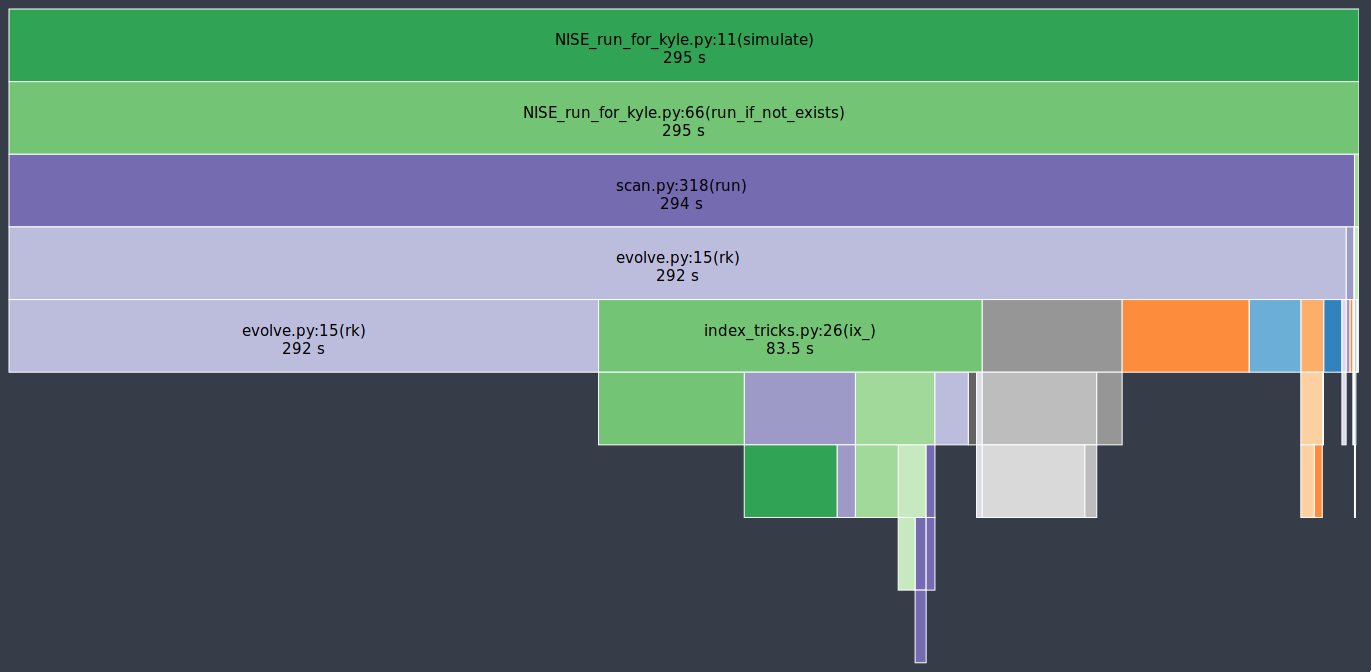
\includegraphics[width=8in]{simulation/images/NISE_prof.png}
\caption{Profile trace of a single threaded simulation from
\texttt{NISE}. \label{sim:fig:snakeviz}}
\end{figure}
\end{landscape}

\begin{landscape}
\begin{figure}
\centering
	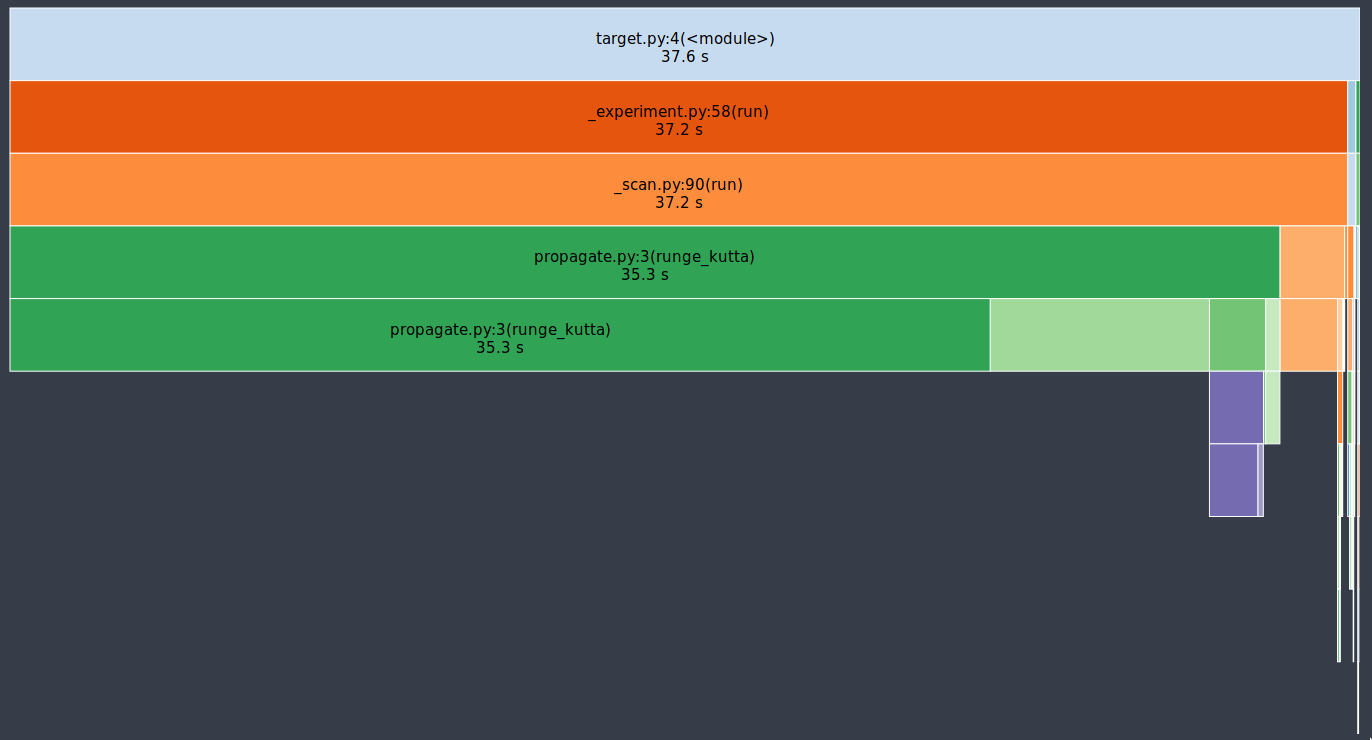
\includegraphics[width=8in]{simulation/images/WrightSim_prof.png}
\caption{Profile trace of a single threaded simulation from
\texttt{WrightSim}. \label{sim:fig:snakeviz2}}
\end{figure}
\end{landscape}

\hypertarget{cpu-and-gpu-parallel-implementations}{%
\paragraph{CPU and GPU Parallel
Implementations}\label{cpu-and-gpu-parallel-implementations}}

\texttt{NISE} already had, and \texttt{WrightSim} inherited, CPU
multiprocessed parallelism using the Python standard library
multiprocessing interface. Since almost all of the program is
parallelizable, this incurs a four times speedup on a machine with four
processing cores (limited more by the operating system scheduling other
tasks than by Amdahl's law). This implementation required little
adjustment outside of minor API tweaks.

In order to capitalize on the highly parallelizable nature of our
multidimensional simulation, the algorithm was re-implemented using
Nvidia CUDA \cite{Nickolls_2008}. In order to make the implementation
as easy to use as possible, and maintainable over the lifetime of
\texttt{WrightSim}, \texttt{PyCUDA} \cite{Klockner_2012} was used to
integrate the call to a CUDA kernel from within Python. \texttt{PyCUDA}
allows the source code for the device side functions (written in C/C++)
to exist as strings within the Python source files. These strings are
just-in-time compiled (using \texttt{nvcc}) immediately prior to calling
the kernel. For the initial work with the CUDA implementation, only one
Hamiltonian and one propagation function were written, however it is
extensible to additional methods. The just-in-time compilation makes it
easy to replace individual functions as needed (a simple form of
metaprogramming).

The CUDA implementation is slightly different from the pure Python
implementation. It only holds in memory the Hamiltonian matrices for the
current and next step, where the Python implementation computes all of
the matrices prior to entering the loop. This was done to conserve
memory on the GPU. Similarly, the electric fields are computed in the
loop, rather than computing all ahead of time. These two optimizations
reduce the memory overhead, and allow for easier to write functions,
without the help of NumPy to perform automatic broadcasting of shapes.

\hypertarget{scaling-analysis}{%
\paragraph{Scaling Analysis}\label{scaling-analysis}}

Scaling analysis, tests of the amount of time taken by each simulation
versus the number of points simulated, were conducted for each of the
following: \texttt{NISE} single threaded, \texttt{NISE} Multiprocessed
using four cores, \texttt{WrightSim} Single threaded, \texttt{WrightSim}
Multiprocessed using four cores, and \texttt{WrightSim} CUDA
implementation. A machine with an Intel Core i5-7600 (3.5 GHz) CPU and
an Nvidia GTX 1060 (3GB) graphics card, running Arch Linux was used for
all tests. The simulations were functionally identical, with the same
number of time steps and same recorded values. The \texttt{NISE}
simulations use two seven by seven matrices for the Hamiltonian, while
the \texttt{WrightSim} simulations use a single nine by nine matrix. The
results are summarized in Figure \ref{sim:fig:scaling}.

\begin{figure}
\centering
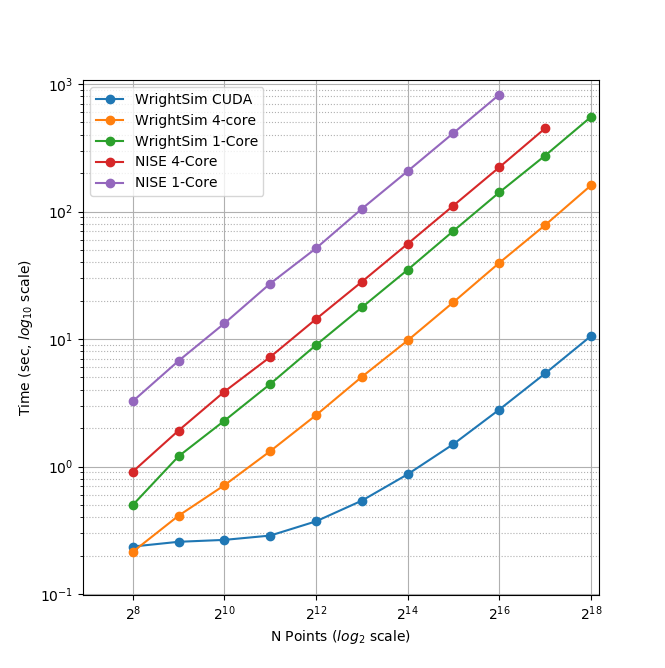
\includegraphics{simulation/images/Scaling.png}
\caption{Scaling Comparison of \texttt{WrightSim} and \texttt{NISE}
\label{sim:fig:scaling}}
\end{figure}

The log-log plot shows that the time scales linearly with number of
points. All lines have approximately the same slope at high values of N,
though the CUDA implementation grows slower at low N. The Algorithmic
improvements alone offer doubled performance over even 4-Core
multiprocessed \texttt{NISE} simulation. The CUDA implementation has a
positive intercept at approximately 200 milliseconds. This is due, in
large part, to the compilation overhead.

\hypertarget{limitations}{%
\paragraph{Limitations}\label{limitations}}

The CUDA implementation faces limitations at both ends in terms of
number of points. On the low side, the cost of compilation and transfer
of data makes it slower than the 4-Core CPU Multiprocessing
implementation. This crossover point is approximately 256 points (for
this simulation, all other parameters being equal). Incidentally, that
is also a hard coded block size for the CUDA kernel call. While this
could be modified to ensure no illegal memory accesses occur on smaller
cases, the fact that you are not saving by using CUDA (and even single
core performance is under a second) means it is not worth the effort at
this time. The hard-coded block size also means that multiples of 256
points must be used in the current implementation.

With larger number of points, we are limited by the amount of memory
available to be allocated on the GPU. For each pixel in the simulations
presented here, 250 complex numbers represented as doubles must be
allocated. Additional space is needed, however it is dominated by this
array, which contains the outputs which are then transferred back to the
host. Each CUDA thread additionally dynamically allocates the arrays it
needs to perform the computation. The current implementation, paired
with the particular hardware used, has a limit somewhere between
\(2^{18}\) and \(2^{19}\) points. This limit could be increased by using
single precision floating point numbers to represent the complex arrays,
if the precision trade-off is acceptable (which is yet to be
determined).

\hypertarget{future-work}{%
\subsubsection{Future Work}\label{future-work}}

This is still quite early days for \texttt{WrightSim}. While it is
already a promising proof of concept display of how \texttt{PyCUDA} can
be applied to this problem, there is still much room for improvement. In
general, there are improvements to be made in terms of features,
API/ease of use, and indeed further algorithmic improvements.

\hypertarget{features}{%
\paragraph{Features}\label{features}}

\texttt{NISE} had implemented a few additional features which were not
carried over to \texttt{WrightSim} during the initial development
efforts which focused on performance thus far.

There was support for chirped electric field pulses, which behave in
less ideal fashions than the true sinusoids and Gaussian peaks used thus
far. These non-ideal perturbations can have a real effect in spectra
collected in the lab, and accurately modelling them helps to interpret
these spectra.

Samples in laboratory experiments may have some amount of inhomogeneity
within the sample, resulting in broader than would otherwise be expected
peaks. This inhomogeneity can be modeled by storing the response array
which is calculated by numerical integration, and translating the points
slightly. The original \texttt{NISE} implementation would perform the
simulation multiple times, where that is not needed as a simple
translation will do. At one point we considered generating a library of
responses in well known coordinates and saving them for future use,
avoiding the expensive calculation all together. That seems to be less
urgent, given the speed of the CUDA code.

\texttt{NISE} provided a powerful and flexible set of tools to
``Measure" the signal, using Fourier transforms and produce arrays that
even further mimic what is observed experimentally. That system needs to
be added to \texttt{WrightSim} for it to be feature-complete. More naïve
methods of visualizing work in this case, but a true measurement would
allow for richer, more detailed analysis and interpretation.

Some new features could be added, including saving intermediate
responses using an HDF5 based file format. The CUDA implementation
itself would benefit from some way of saving the compiled code for
multiple runs, removing the 0.2 second overhead. Current implementation
compiles directly before calling the kernel, whether it has compiled it
before or not. If performing many simulations in quick succession (e.g.
a simulation larger than the memory allows in a single kernel call) with
the same C code, the savings would add up.

The just-in-time compilation enables some special metaprogramming
techniques which could be explored. The simple case is using separately
programmed functions which have the same signature to do tasks in
different ways. Currently there is a small shortcut in the propagation
function which uses statically allocated arrays and pointers to those
arrays rather than using dynamically allocated arrays. This relies on
knowing the size at compilation time. The numbers could be replaced by
preprocessor macros which are also fed to the compiler to assign this
value "pseudo-dynamically" at compilation time. A much more advanced
metaprogramming technique could, theoretically, generate the C struct
and Hamiltonian generation function by inspecting the Python code and
performing a translation. Such a technique would mean that new
Hamiltonians would only have to be implemented once, in Python, and
users who do not know C would be able to run CUDA code.

\hypertarget{usability}{%
\paragraph{Usability}\label{usability}}

One of the primary reasons for reimplementing the simulation package is
to really think about our interface. As much as possible, the end user
should not need to be an experienced programmer to be able to get a
simulation. One of the next steps for \texttt{WrightSim} is to take a
step back and ensure that our API is sensible and easy to follow. We
wish to, as much as possible, provide ways of communicating through
configuration files, rather than code. Ultimately, a GUI front end may
be desirable, especially as the target audience is primarily
experimentalists.

Additional Hamiltonians would make the package significantly more
valuable as well. To add more Hamiltonians will require ensuring the
code is robust, that values are transferred as expected. A few small
assumptions were made in the interest of efficiency in the original
implementation. Certain values, such as the initial density vector,
represented by the Hamiltonian were hard-coded on the device code. While
the hard-coded values are reasonable for most simulations, the ability
to set theses at run time is desired, and will be added in the future.

\hypertarget{further-algorithmic-improvements}{%
\paragraph{Further Algorithmic
Improvements}\label{further-algorithmic-improvements}}

While great strides were taken in improving the algorithms from previous
implementations, there are several remaining avenues to gain improved
performance in execution time and memory usage. The CUDA implementation
is memory bound, both in terms of what can be dispatched, and in terms
of time of execution. The use of single precision complex numbers (and
other floating point values) would save roughly half of the space. One
of the inputs is a large array with parameters for the each electric
field at each pixel. This array contains much redundant data, which
could be compressed with the parsing done in parallel on the device.

If the computed values could be streamed out of the GPU once computed,
while others use the freed space, then there would be almost no limit on
the number of points. This relies on the ability to stream data back
while computation is still going, which we do not have experience doing,
and are not sure CUDA even supports. The values are not needed once they
are recorded, so there is no need from the device side to keep the
values around until computation is complete.

Additional memory could be conserved by using a bit field instead of an
array of chars for determining which time orderings are used as a
boolean array. This is relatively minimal, but is a current waste of
bits. The Python implementation could potentially see a slight
performance bump from using a boolean array rather than doing list
searches for this same purpose.

The CUDA implementation does not currently take full advantage of shared
cache. Most of the data needed is completely separated, but there are
still a few areas where it could be useful.

The current CUDA implementation fills the Hamiltonian with zeros at
every time step. The values which are nonzero after the first call are
always going to be overwritten anyway, so this wastes time inside of of
nested loop. This zeroing could be done only before the first call,
removing the nested loop. Additionally, many matrices have a lot of zero
values. Often they are triangular matrices, which would allow for a more
optimized dot product computation which ignores the zeros in the half
which is not populated. Some matrices could even benefit by being
represented as sparse matrices, though these are more difficult to use.

Finally, perhaps the biggest, but also most challenging, remaining
possible improvement would be to capitalize on the larger symmetries of
the system. It's a non-trivial task to know which axes are symmetric,
but if it could be done, the amount that actually needs to be simulated
would be much smaller. Take the simulation in Figure
\ref{sim:fig:examplespectrum}. This was computed as it is displayed, but
there are two orthogonal axes of symmetry, which would cut the amount
actually needed to replicate the spectrum down by a factor of four.
Higher dimensional scans with similar symmetries would benefit even
more.

\hypertarget{conclusions}{%
\subsubsection{Conclusions}\label{conclusions}}

\texttt{WrightSim}, as implemented today, represents the first major
step towards a cohesive, easy to use, fast simulation suite for quantum
mechanical numerically integrated simulations using density matrix
theory. Solely algorithmic improvements enabled the pure Python
implementation to be an order of magnitude faster than the previous
implementation. The algorithm is highly parallelizable, enabling easy
CPU level parallelism. A new implementation provides further improvement
than the CPU parallel code, taking advantage of the General Purpose-GPU
Computation CUDA library. This implementation provides approximately 2.5
orders of magnitude improvement over the existing \texttt{NISE} serial
implementation. There are still ways that this code can be improved,
both in performance and functionality. With \texttt{WrightSim}, we aim
to lead by example among the spectroscopic community by providing an
open-source package for general-purpose MDS simulation.


\clearpage
